%% LaTeX file for Design representation
%% design.tex
%% 
%% Karlsruhe Institute of Technology
%% Version 1.0, 2018-12-13

%% Available page modes: oneside, twoside
%% Available languages: english, ngerman
%% Available modes: draft, final (see README)
\documentclass[twoside, english, draft]{design}

\usepackage{graphicx}
\usepackage{caption}
\usepackage{pdfpages}
\usepackage[export]{adjustbox}

%usepackage{lipsum}


%% ---------------------------------
%% | Information about the thesis  |
%% ---------------------------------

%% Name of the author
\author{PSE Group}

%% Title (and possibly subtitle) of the thesis
\title{
Design}

%% Type of the thesis 
\thesistype{PSE}

%% The advisors are PhD Students or Postdocs
\advisor{M.Sc. Ankush Meshram}
%\begin{document}


%\end{document}
\thispagestyle{empty}

\settitle

%% --------------------------------
%% | Settings for word separation |
%% --------------------------------

%% Describe separation hints here.
%% For more details, see 
%% http://en.wikibooks.org/wiki/LaTeX/Text_Formatting#Hyphenation
\hyphenation{
% me-ta-mo-del
}

%% --------------------------------
%% | Bibliography                 |
%% --------------------------------

%% Use biber instead of BibTeX, see README
\usepackage[citestyle=numeric,style=numeric,backend=biber]{biblatex}
\usepackage{microtype}

\addtolength{\belowcaptionskip}{-10pt}
\setlength{\textfloatsep}{10pt plus 1.0pt minus 2.0pt}
%\addtolength{\abovecaptionskip}{-100pt}
\frenchspacing
%% ====================================
%% ====================================
%% ||                                ||
%% || Beginning of the main document ||
%% ||                                ||
%% ====================================
%% ====================================
\begin{document}
\nocite{*}

%% Set PDF metadata
\setpdf

%% Set the title
\maketitle

%% ----------------
%% |   Abstract   |
%% ----------------

%% The text is included from the following files:
%% - sections/abstract
\thispagestyle{empty}
\begin{abstract}
\thispagestyle{empty}
\end{abstract}

%% -----------------
%% |   Main part   |
%% -----------------
\thispagestyle{empty}
\newpage
\thispagestyle{empty}
\tableofcontents
\cleardoublepage
\setcounter{page}{1}


\section{Design}\label{sec:intro}
\subsection{Front-End}
\subsubsection{Sequence Diagram}



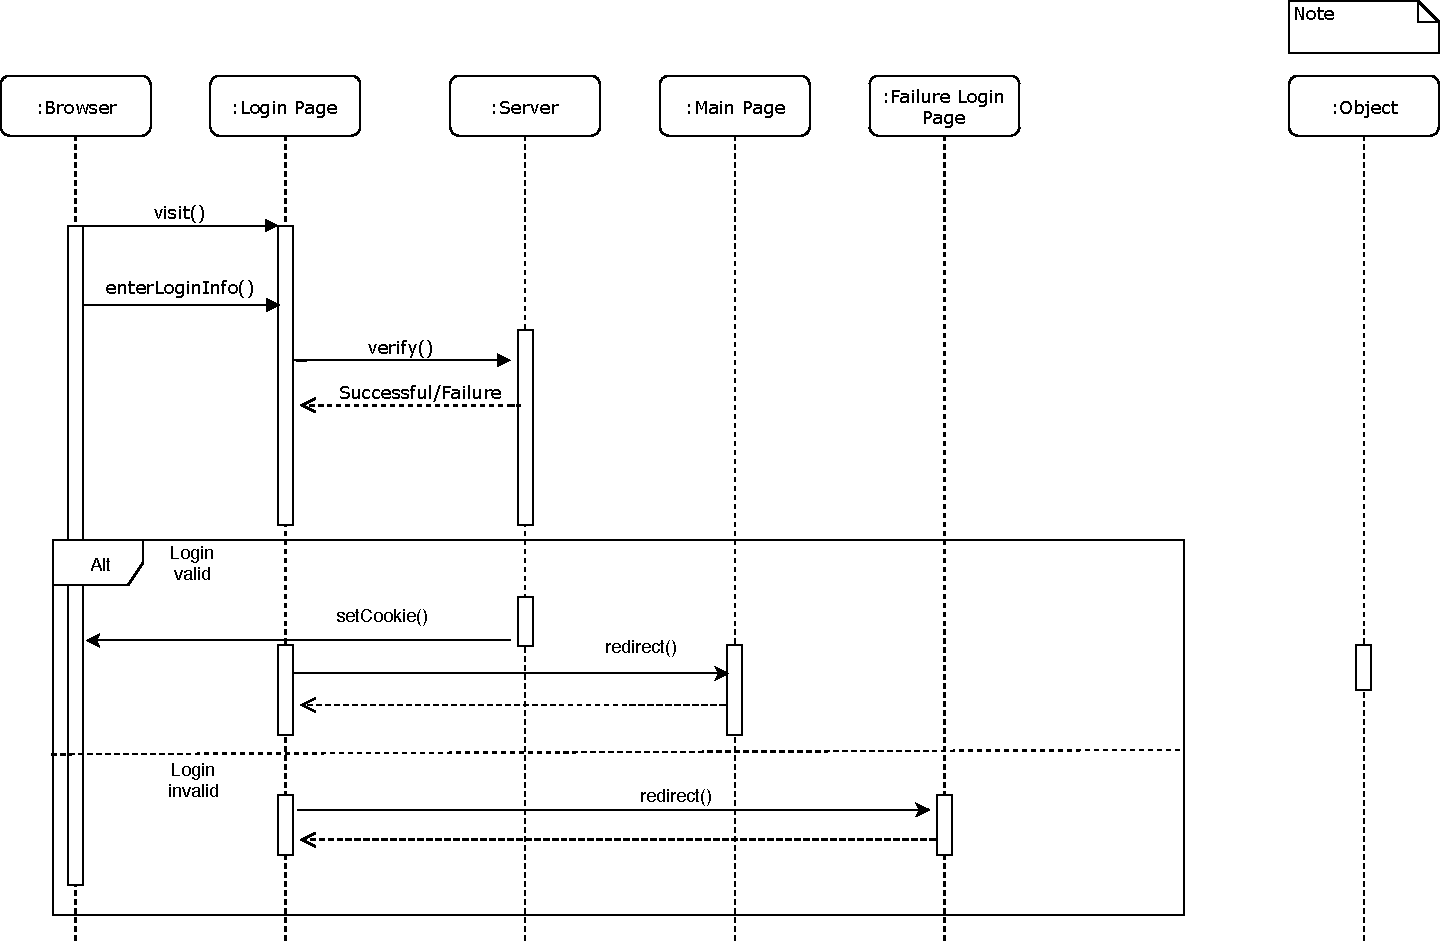
\includegraphics[max size={\textwidth}{\textheight}]{login1.pdf}
\newpage
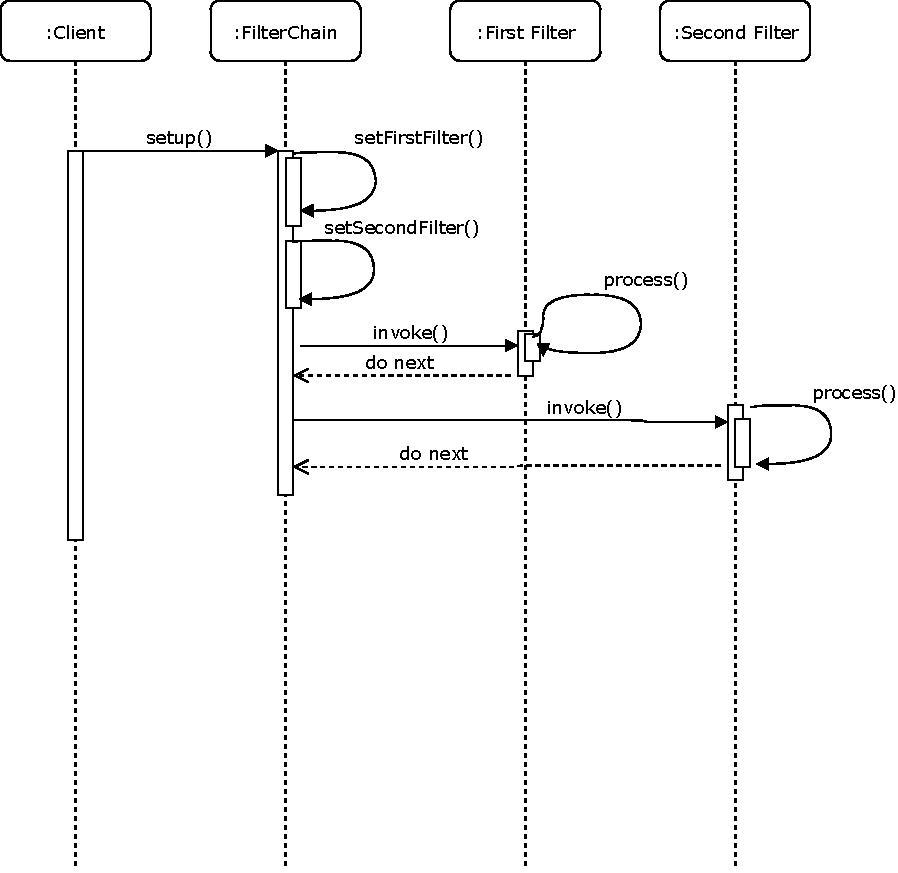
\includegraphics[max size={\textwidth}{\textheight}]{filterchain.pdf}
\newpage
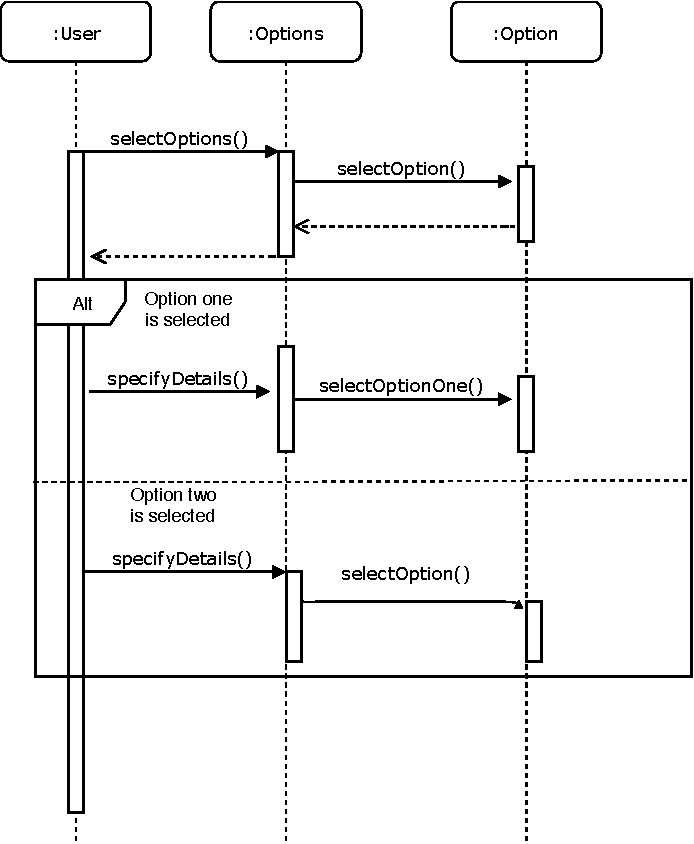
\includegraphics[max size={\textwidth}{\textheight}]{option.pdf}

\subsubsection{Activity Diagram}
\subsubsection{Class Diagram}
\newpage
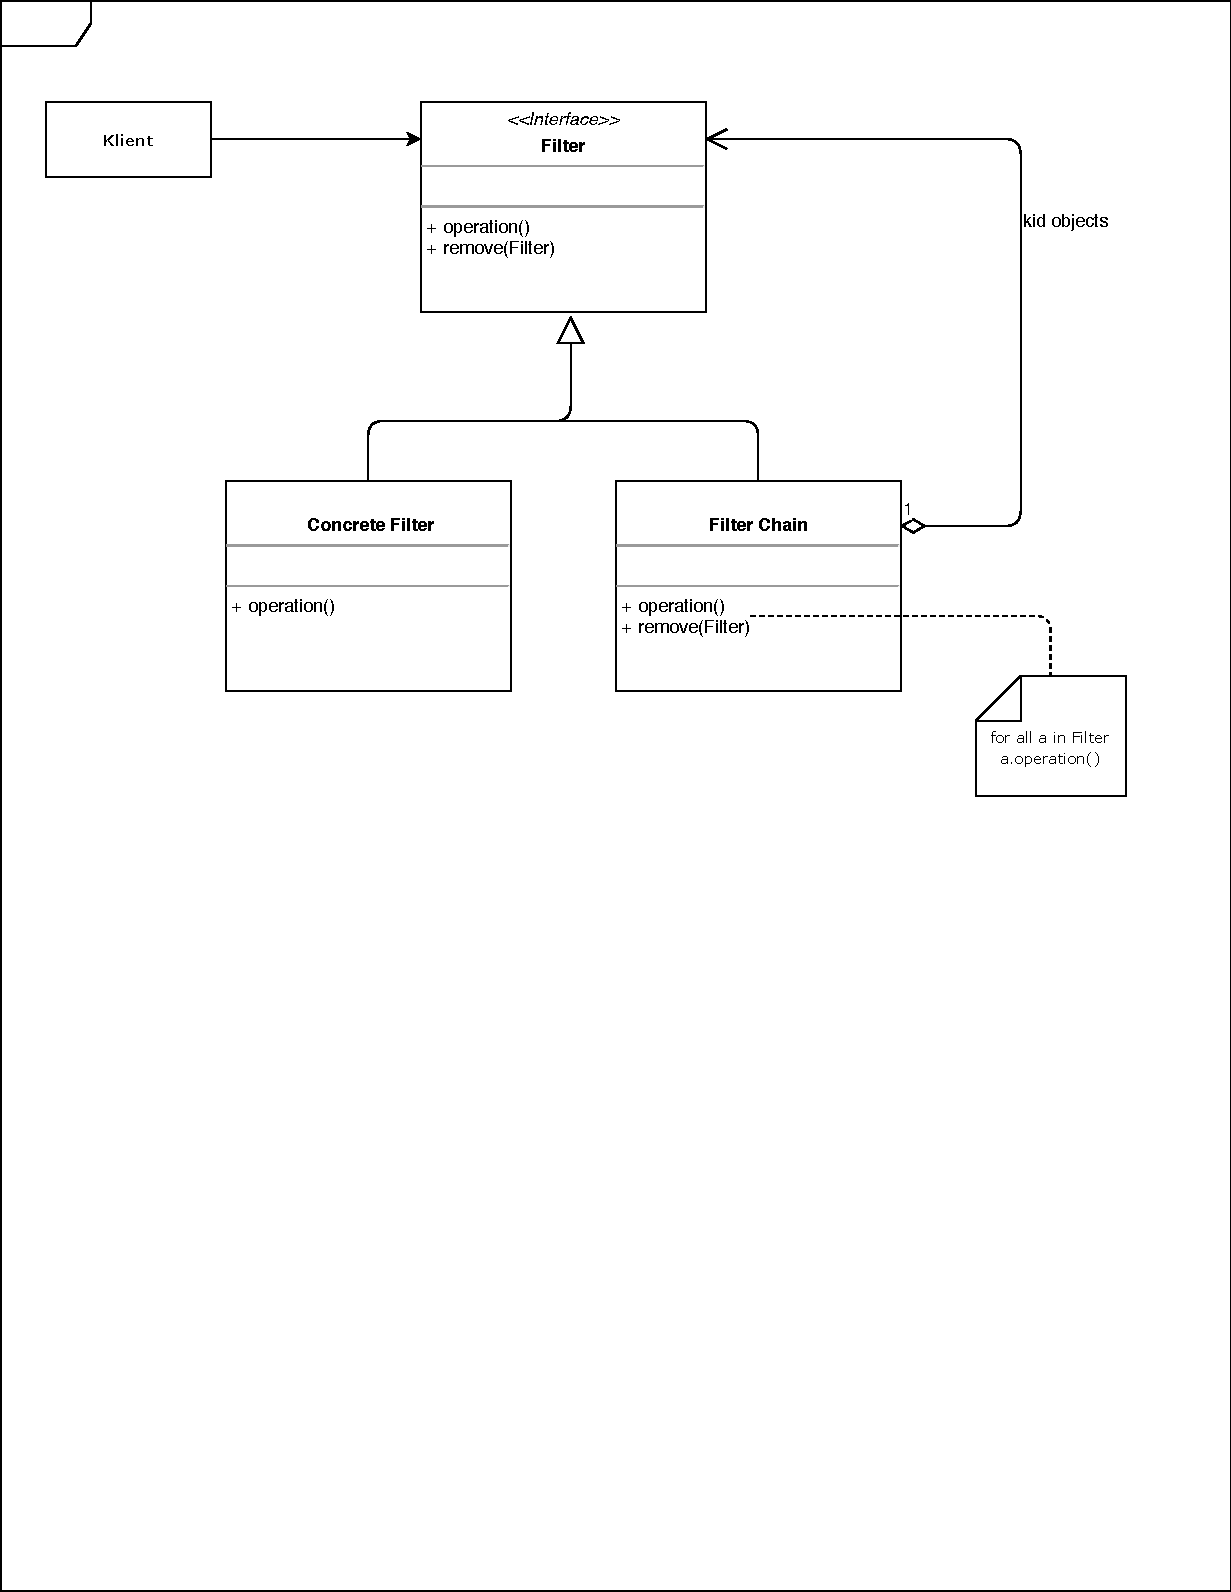
\includegraphics[max size={\textwidth}{\textheight}]{filterclassdiagram.pdf}
\newpage
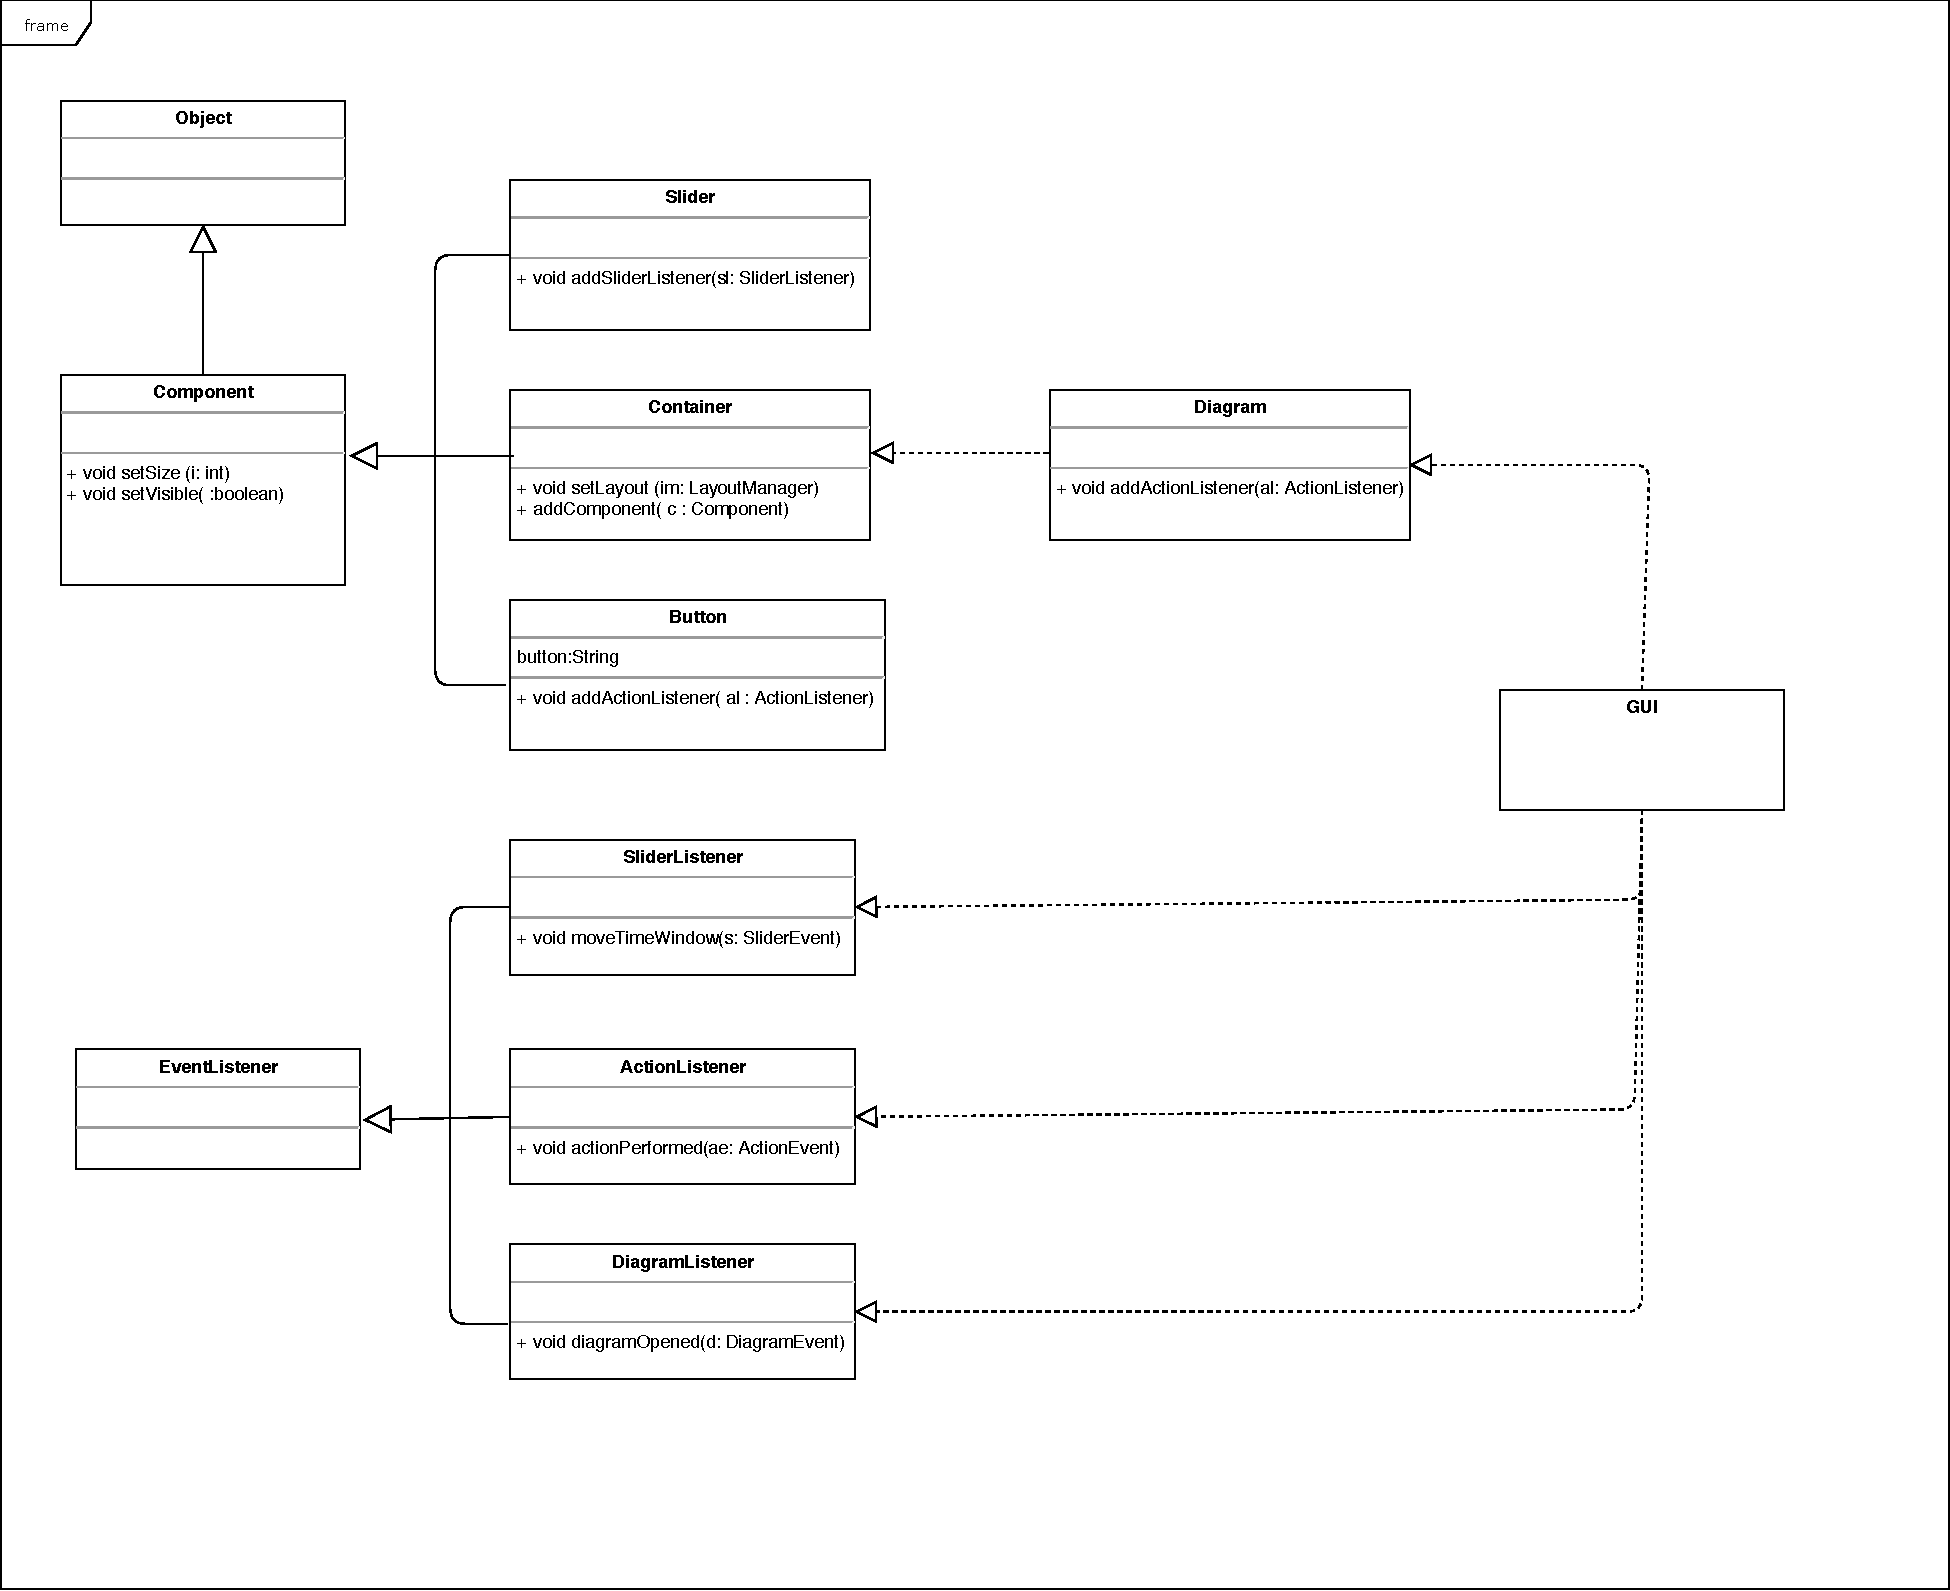
\includegraphics[max size={\textwidth}{\textheight}]{frame.pdf}
\newpage
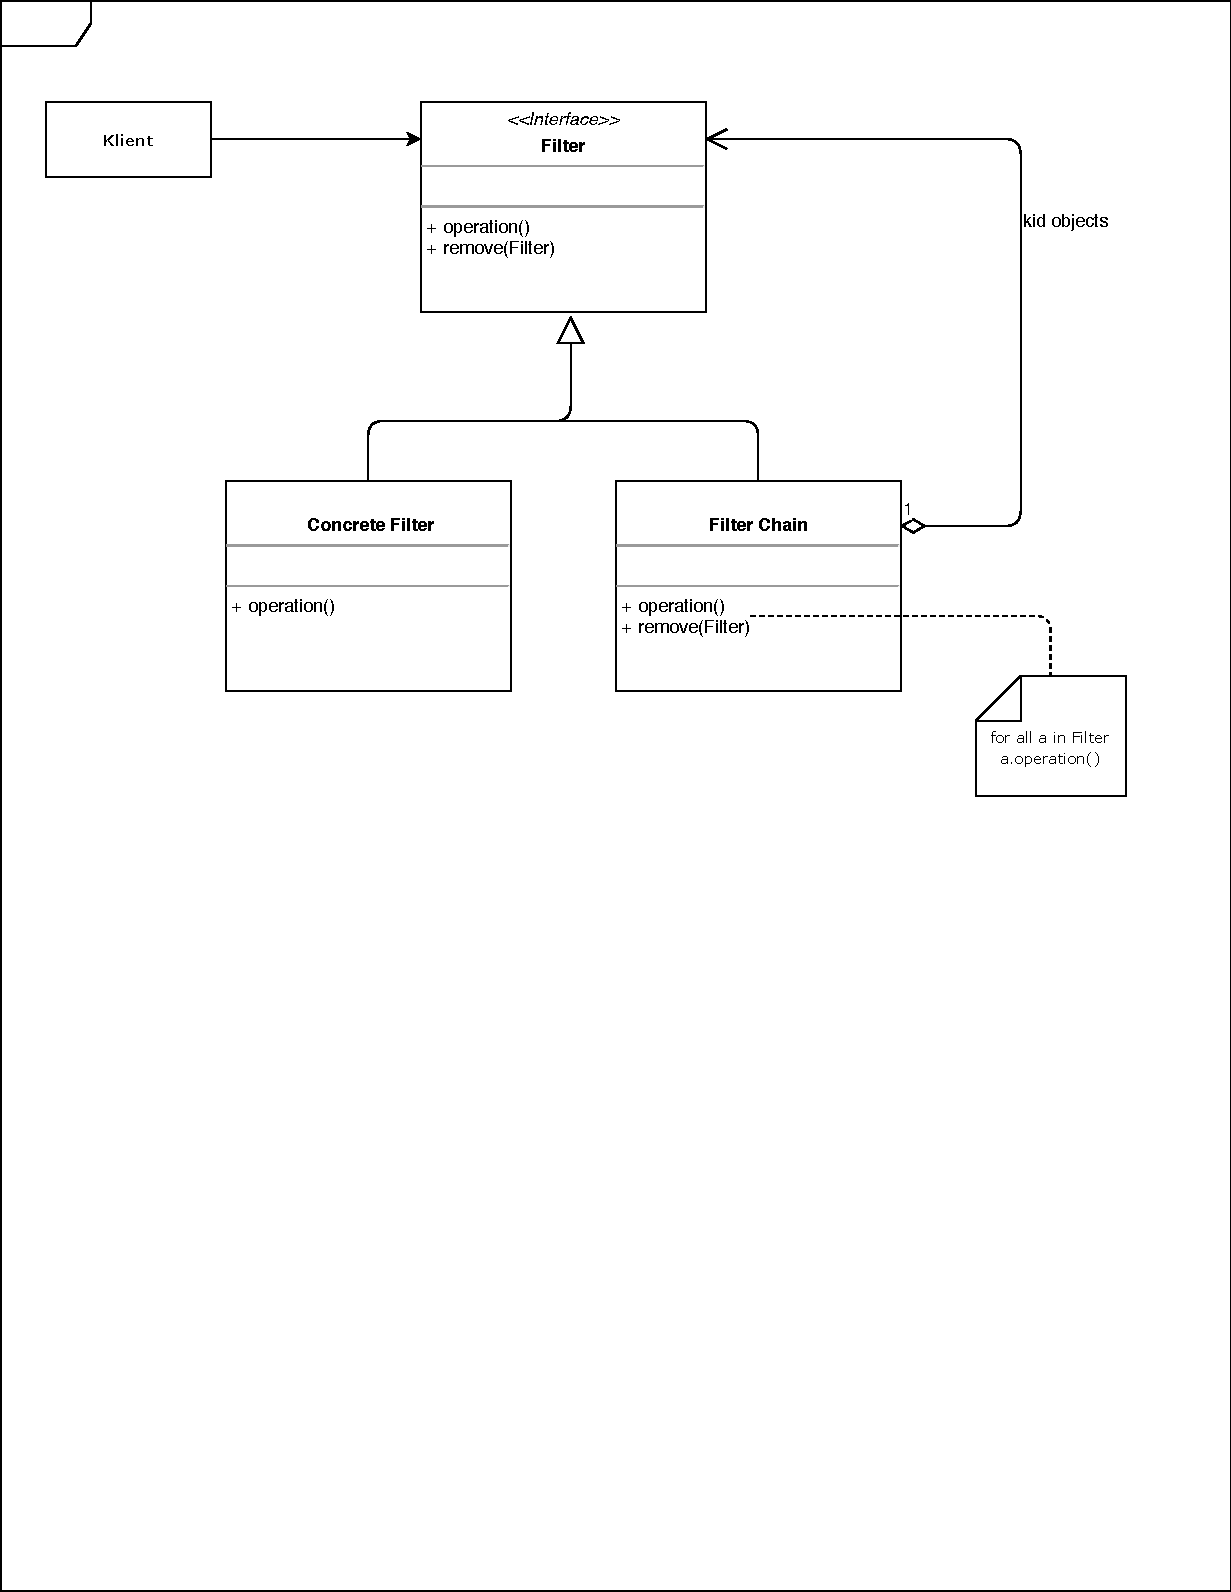
\includegraphics[max size={\textwidth}{\textheight}]{login2.pdf}

\subsection{Back-End}
\subsubsection{Sequence Diagram}
\subsubsection{Activity Diagram}
\subsubsection{Class Diagram}


\end{document}